\section{Concurrency management}

\begin{figure}[h!]
		\centering
		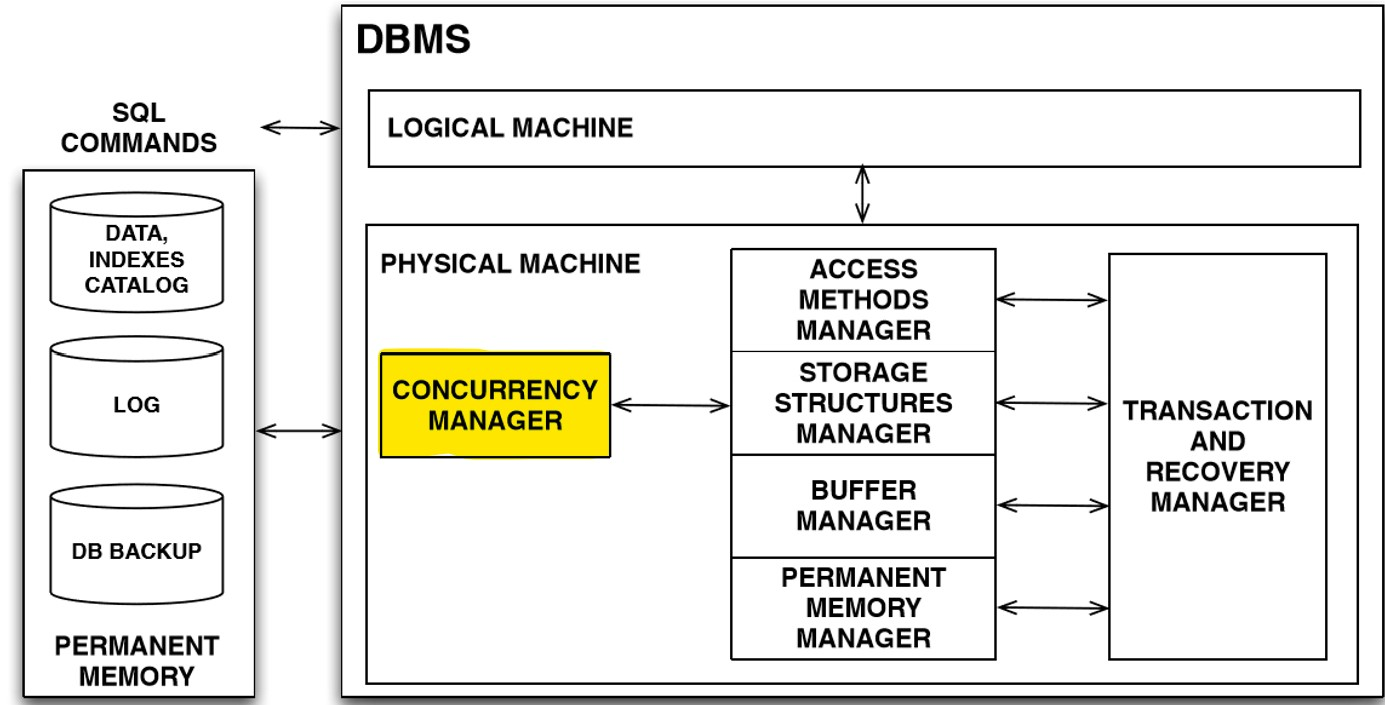
\includegraphics[scale = 0.7]{img/conc1.jpg}
		\label{tr10}
\end{figure}

When executing concurrent transactions, some interference may leave the DB in an inconsistent state. The \textit{Concurrency Manager} is the system module that ensures the execution of concurrent transactions without interference during DB access.

\subsection{Introduction}
The problem about concurrent transactions is that their database operations are interleaved, i.e. operations from one program can execute in between operations from another program. This interleaving can cause programs to produce unpredictable results

Assuming that each transaction is \textit{consistent}, a simple way to avoid interference among concurrent transactions is to allow only a \textbf{serial execution}  of them, i.e. all the operations of a transaction are executed before any operation of the other. However, serial executions are impractical from a performance perspective, so we consider a \textbf{serializable execution}. An execution of a set of transactions is \textit{serializable} if its effect is exactly the same as a serial execution of the committed transactions. Serializable executions are \textbf{correct}, because each serializable execution has the same effect of a serial one, and serial executions are correct.

In this sense, the goal of the \textit{Concurrency Manager} is to establish an order among the operations of a set of transactions to make its execution serializable. Its correctness is proved by using the results of the \textbf{serializability theory}, which uses a structure called \textbf{history} (or \textbf{schedule}) to represent the chronological order in which the operations of a set of concurrent transactions are executed, and which goal is to define the properties that an history has to hold to be serializable.

\subsection{Histories}
From the DBMS's point of view, a transaction is seen as a set of read/write/commit and abort operations. For example, this program:

\begin{figure}[h!]
		\centering
		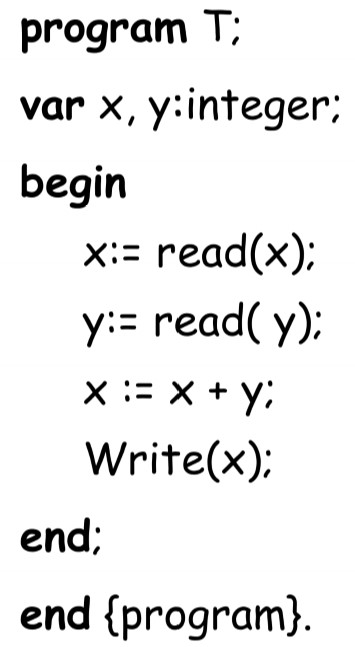
\includegraphics[scale = 0.7]{img/conc2.jpg}
		\label{tr10}
\end{figure}

is seen as $r_1[x]$, $r_1[y]$, $w_1[x]$, $c_1$. 

We make the following assumptions:

\begin{itemize}

    \item a transaction is a set of read/write operations which terminates only with a commit or an abort;
    
    \item we do not consider the operations of insertion or deletion of records;

    \item a transaction reads/writes a specific record at most once.
    
\end{itemize}

We now introduce the concept of history:

\begin{tcolorbox}

 Let $T = \{T_1, T_2, ..., T_n\}$ a set of transaction. A \textbf{history} (or \textbf{schedule}) $H$ on $T$ is an ordered set of operations such that: 

 \begin{enumerate}
     \item the operation of $H$ are those of $T_1, T_2, ..., T_n$
     \item $H$ preserves the ordering between the operations belonging to the same transaction
 \end{enumerate}


\end{tcolorbox}

Intuitively, the history $H$ represents the actual or potential execution order of the operations of the transactions $T_1, T_2, ..., T_n$. An example of history involving three transactions could be the following one:

\begin{figure}[h!]
		\centering
		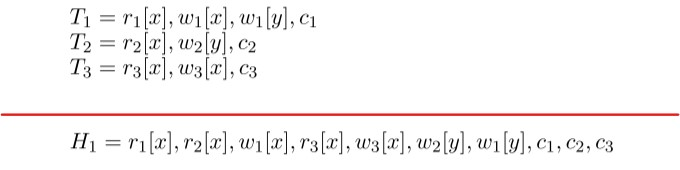
\includegraphics[scale = 1.5]{img/conc3.jpg}
		\label{tr10}
\end{figure}

\subsubsection{Equivalent histories}

For \textbf{equivalent histories} we could mean that they produce the same effects on the database, namely that the values written to the database by the committed transactions are equal. Since a DBMS knows nothing of the computations made by a transaction in temporary memory, a \textbf{weaker notion} of equivalence which takes into account only the order of operations in conflict made on the database is preferred.

\begin{tcolorbox}
    Two operations of different transactions are in \textbf{conflict} if they are on the same data item and at least one of them is a write operation.
\end{tcolorbox}

This definition allows us to define three types of situations in which the operations are in conflict:

\begin{itemize}

    \item Write-Read Conflict. \\Consider the following piece of a history: $H = ...w1[x],r2[x]...$. The transaction $T_2$ reads $x$ updated by $T_1$ which has not yet committed. This type of read, called \textit{dirty read}, can give rise to executions not serializable;

    \item Read-Write Conflict. \\Consider the following piece of a history: $H = ...r1[x],w2[x],r1[x],...$ Transaction $T_2$ writes a data $x$ previously read by the transaction $T_1$, still active, which then rereads it getting a different value even if in meanwhile $T_1$ has not updated it. This effect obviously can not be achieved by any serial execution of the two transactions;

    \item Write-Write Conflict. \\Consider the following piece of a history: $H = ...w1[x],w2[x]...$ The two transactions, while attempting to modify a data item $x$, both have read the item’s old value before either of them writes the item’s new value. 
    
\end{itemize}

\begin{tcolorbox}
    Two histories $H_1$ and $H_2$ are \textbf{c-equivalent} (conflict-equivalent), i.e. equivalent with respect to operations in conflict, if:
    
    \begin{enumerate}
        \item they are defined on the same set of transactions $T = \{T_1, T_2, ..., T_n\}$ and have the same operations;
        \item they have the same order of operations in conflict of transactions terminated normally
    \end{enumerate}
    
\end{tcolorbox}

Condition (1) requires that $H_1$ and $H_2$ contain the same set of operations to be comparable, while condition (2) requires that $H_1$ and $H_2$ have the same order of the operations in conflict of committed transactions

\subsection{Serializable history}
A history $H$ on the set $T = \{ T_1, T_2, ..., T_n \}$ is \textbf{serial} if it represents a serial execution of $T$ in some order. 

We can now define a stronger condition that is sufficient to ensure that a history is serializable:

\begin{tcolorbox}
    A history $H$ on the transactions $T = \{T_1, T_2, ..., T_n\}$ is \textbf{c-serializable} if it is c-equivalent to a serial history on $T_1, T_2, ..., T_n$.
\end{tcolorbox}

\textbf{NOTE} that each c-serializable history is serializable, but there are serializable histories that are not c-serializable.

\paragraph{Serialization graph}
Another way of examining a history $H$ and decide whether it is c-serializable or not is to analyze a particulare graph derived from $H$, called the \textbf{serialization graph}.

\begin{tcolorbox}
    Let $H$ be a history of committed transactions $T = \{T_1, T_2, ..., T_n\}$. The \textbf{serialization graph} of $H$, denoted $SG(H)$, is a directed graph such as:
    \begin{itemize}
        \item there is a node for every committed transaction in $H$;
        \item there is a directed arc from $T_i \rightarrow T_j$, with $(i \neq j)$ if and only if in $H$ some operation $p_i$ in $T_i$ appears before and conflicts with some operation $p_j$ in $T_j$.
    \end{itemize}

\end{tcolorbox}

We say that two transactions $T_i$ and $T_j$ conflicts if $T_i \rightarrow T_j$ appears in $SG(H)$.

As an example, this is the serialization graph of the given history.

\begin{figure}[h!]
		\centering
		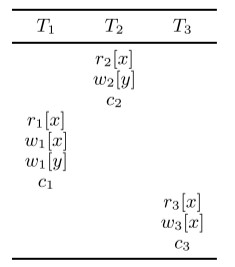
\includegraphics[scale = 1.5]{img/conc4.jpg}
		\label{conc4}
\end{figure}

\begin{figure}[h!]
		\centering
		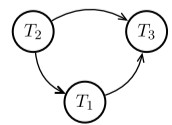
\includegraphics[scale = 1.5]{img/conc5.jpg}
		\label{conc5}
\end{figure}

\begin{tcolorbox}[title = C-Serializability theorem]
    A history $H$ is c-serializable if and only if its serialization graph $GS(H)$ is acyclic.
\end{tcolorbox}

Since Picture \ref{conc5} represents an acyclic graph, the history in Picture \ref{conc4} is c-serializable!

\subsection{Serializability with locking}

From the analysis of the serialization graph it can be verified a posteriori if a history is c-serializable. Histories and serialization graphs, however, are abstract concepts, and during the execution of a set of transactions, the \textbf{serialization graph is not constructed}. Conversely, the c-serializability theorem is used to prove that the \textbf{scheduling algorithm for the concurrency control} used by a scheduler is correct, i.e. that all histories representing executions that could be produced by it are c-serializable.

\subsubsection{Strict two-phase locking}
A simple scheduling algorithm to obtain serializability is the \textit{Strict 2PL} protocol. The idea behind this approach is simple: each data item used by a transaction has a \textbf{lock} associated with it, which could be:

\begin{itemize}
    \item a \textit{read} or \textit{shared} (S) lock;
    \item a \textit{write} or \textit{exclusive} (X) lock.
\end{itemize}

, and it follows two rules:

\begin{enumerate}

    \item if a transaction $T_i$ wants to read a data item, it first request a shared lock on the data item (first phase):
    
    \begin{itemize}
    
        \item if no other transaction holds the lock, then the data item is locked;
        
        \item if another transaction $T_j$ holds a lock in conflict, then $T_i$ must wait until $T_j$ releases it
        
    \end{itemize}

    
    \item All locks held by a transaction $T_i$ are released together when $T_i$ commits or aborts (second phase). To guarantee the isolation of a transaction, lock releases cannot occur before commit/abortion time.
   
\end{enumerate}

We can describe the \textit{lock-granting policies} of Strict 2PL protocol using a \textbf{compatibility matrix}: 

\begin{itemize}

    \item a row corresponds to a lock that is already held on an element $x$ by another transaction;
    
    \item the columns correspond to the mode of lock on $x$ that is requested
    
\end{itemize}

\begin{figure}[h!]
		\centering
		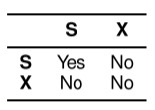
\includegraphics[scale = 1.5]{img/conc6.jpg}
		\label{conc5}
\end{figure}

\textbf{NOTE}: 
\begin{itemize}

    \item requests to acquire or release locks are automatically inserted into transactions by the \textit{Transaction Manager};
    
    \item lock and unlock requests are handled by the scheduler with the use of the \textit{Lock Table}, in which an entry contains the ID of the data item being blocked, the type of lock granted or requested, a list of transactions holding lock and a queue of lock requests.
    
\end{itemize}

\begin{tcolorbox}[title = C-Serializability of Strict 2PL]
    A \textit{Strict 2PL} protocol ensures c-serializability.
\end{tcolorbox}

However, the set of \textit{Strict 2PL} histories is a subset of the c-serializable histories, i.e. there are c-serializable histories that are not \textit{Strict 2PL}.

\subsubsection{Deadlocks}

Although being simple, \textit{Strict 2PL} needs a strategy to detect \textit{deadlocks}, a situation in which, for example, two transactions lock two different items and none of them can proceed. The deadlock problem can be solved with deadlock prevention techniques or with deadlock detection and recovery technques.

\paragraph{Deadlock detection}

\begin{itemize}

    \item a strategy to detect deadlocks uses a \textbf{wait-for graph}, in which :
    
    \begin{itemize}
    
        \item the nodes are active transactions;
        
        \item an arc from $T_i$ to $T_j$ indicates that $T_i$ is waiting for a resource held by $T_j$.

    \end{itemize}  
    
    Using this representation, a \textbf{cycle} in the graph indicates that a \textbf{deadlock} has occurred, and one of the transactions of the cycle must abort;
    
    \item the standard method to decide which transaction to abort is to choose the \textbf{“youngest”} transaction by some metric (being young, it has probably done less work, so it is less costly to abort);
    
    \item checking for cycles requires a linear complexity algorithm, but the actual cost of the management of the graph in real cases discourage the use. For this reason, instead of wait-for graph we can use the \textbf{timeout strategy}: if a transaction has been waiting too long for a lock, then the scheduler simply presumes that deadlock has occurred and it aborts the transaction.

\end{itemize}

\paragraph{Deadlock prevention}

\begin{itemize}
    \item each transaction $T_i$ receives a timestamp $t_s(T_i)$ when it starts: $T_i$ is older than $T_j$ if $t_s(T_i) < t_s(T_j)$;

    \item each transaction is assigned a priority on the basis of its timestamp: the \textbf{older} a transaction is, the \textbf{higher priority} it has. 
    
    \item when a transaction $T_i$ requests a lock on a data item that conflicts with the lock currently held by another active transaction $T_j$, two algorithms are possible:

    \begin{enumerate}
    
        \item wait-die (or non-preemptive technique): an older transaction waits only for a younger one, otherwise the younger dies.
        
        \item wound-wait (or preemptive technique): an older transaction wounds a younger one to take its lock, otherwise the younger waits for the older one.
        
    \end{enumerate}
    
    
    In both cases when an aborted transaction $T_i$ is restarted, it has the same priority it had originally: this property ensures that sooner or later every transaction will become the oldest, so it ensures that no \textit{starvation} will occur.

    These two algorithms have the property of \textbf{not creating deadlocks}, but their behaviour is very different:

    \begin{itemize}

        \item with the wait-die method, a transaction $T$ can wait for data locked by a younger transaction or it restarts due to an older one $T_0$. Most likely is the second case and then the method favors the restarting rather than waiting;
    
        \item with the wound-wait method, a transaction $T$ can wait for data locked by an older transaction or restarts a younger one $T_y$. Most likely is the first case followed by the waiting rather than restarting.
        
    \end{itemize}

    \item deadlock prevention methods are easier to implement than deadlock detection solutions, but on the other hand they lead to the abortion of transactions which could run without restarts.
    
\end{itemize}

\subsection{Serializability without locking}
While methods of concurrency control that use locks are called \textit{pessimistic}, in the sense that they're based on the idea that a bad things is likely to happen, other methods, called \textit{optimistic}, do not lock data because are based on the idea that bad things are not likely to happen. However, in this approach, when a transaction requests to commit, the system controls that no bad things has happened.

\paragraph{Snapshot isolation}

\begin{itemize}

    \item a transaction can perform any database operation without requesting permission, and taking advantage of \textit{multiversions} of each data item;
    
    \item the transactions must request permission to commit;

    \item each transaction $T_i$ reads the data of the DB version (\textit{snapshot}) produced by all the transactions committed before $T_i$ starts, but no effects are seen of other concurrent transactions. 

    \item this approach grants that no concurrent writes are performed ("First-Committer-Wins" rule).
    
\end{itemize}

\subsection{Multiple granularity locking}
The concurrency control techniques seen so far, based on the idea of a single record lock, is not sufficiently general to treat transactions that operate on collections of records. For example, in some cases it could be convenient to lock an entire table, rather that a single record. 

For this reason, other techniques are base on the idea that the data to lock can have different \textbf{granularities}, and among them is defined an inclusion relationship : $\text{DB} \rightarrow \text{Files} \rightarrow \text{Pages} \rightarrow \text{Records} \rightarrow \text{Fields}$.

The inclusion relation between data can be thought of as a \textbf{tree} of objects where each node contains all its children. If a transaction gets an \textit{explicit} $S$ or $X$ lock on a node, then it has an \textit{implicit} lock in the same lock mode on all the descendants of that node.

In order to manage locks on data of different granularities, \textit{intention locks} are introduced: 

\begin{tcolorbox}[title = Multiple-granularity and intention locks]
    Multiple-granularity locking requires that before a node in explicitly locked, a transaction must first have a proper intention lock on all the ancestors of that node in the granularity hierarchy. 
\end{tcolorbox}

The intention locks are the following:

\begin{itemize}

    \item $IS$, or \textit{intention shared lock}, allows requestor to explicitly lock descendant nodes in $S$ or $IS$ mode;

    \item $IX$ or \textit{intention exclusive lock}, allows requestor to explicitly lock descendants in $S$, $IS$, $X$, $IX$ or $SIX$ mode;
    
    \item $SIX$ or \textit{shared intentional exclusive lock}, implicitly locks all descendants of node in $S$ mode and allows requestor to explicitly lock descendant nodes in $X$, $SIX$, or $IX$ mode.
    
\end{itemize}

Note that the $SIX$ lock is introduced in order to combine $S$ and $IX$ to simplify the lock manager, since they frequently appera together.

The compatibility matrix is:

\begin{figure}[h!]
		\centering
		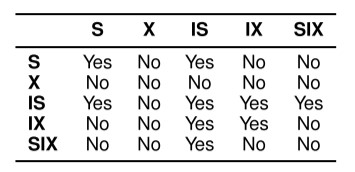
\includegraphics[scale = 1.5]{img/conc7.jpg}
		\label{conc5}
\end{figure}

To deal with multiple granularity locks, it is necessary extend the \textit{Strict 2PL protocol} with new rules, obtaining the protocol called \textbf{Multi-granularity Strict 2PL}:

\begin{enumerate}

    \item a node can be locked by a transaction $Ti$ in $S$ or $IS$ mode only if the parent is locked by $Ti$ in $IS$ or $IX$ mode.
    
    \item a node can be locked by a transaction $Ti$ in $X$, $IX$ or $SIX$ mode only if the parent is locked by $Ti$ in $SIX$ or $IX$ mode.

\end{enumerate}

\subsection{Locking for dynamic databases}

So far we have considered only transactions that read or update existing records in the database. In reality, transactions can also \textbf{insert} or \textbf{delete} records into tables with \textbf{indexes}. These possibilities raise new problems to be solved to ensure serializability during the concurrent execution of a set of transactions, while continuing to adopt the Strict 2PL protocol.

\paragraph{Insertion and Deletion}
The inserted or deleted records are called \textit{phantoms} because they are records that appear or disappear from sets, i.e. they are invisible only during a part of a transaction execution. 

An acceptable practical solution to this problem is \textbf{index locking}. When a set of records that match some predicate is locked, the database system also checks to see if there is an index whose key matches the predicate. If such an index exists, the structure of the index should allow us to easily lock all the pages in which new tuples that match the predicate appear or will appear in the future. The practical issue of how to locate the relevant pages in the index that need to be locked and what locks need to be acquired is discussed in the following section.

\paragraph{Concurrency Control in B+–trees}

The concurrent use of a B+–tree index by several transactions may be treated in a simple way with \textit{Strict 2PL protocol}, by considering each node as a granule to lock appropriately. This solution, however, would lead to a low level of concurrency due to locks on the first tree levels. 

A better solution is obtained by exploiting the fact that the indexes are used in a particular way during the operation. In the case of a search, the nodes visited to reach the leaves, where the data is located, are locked in reading during the visit and unlocked as soon as the search proceeds from one node to the child. In the case of an insertion, during the visit of the tree when switching from one node $A$ to a child $B$ not full, the locks on $A$ can be released because a possible propagation of the effect of the insert into a leaf stops at node $B$, called a (safe node). A node is safe for a delete operation if it is at least half full. The general case with node splits, merging and balancing is more complex and several tree locking techniques have been proposed. 

